\documentclass[12pt]{article}

\usepackage[utf8]{inputenc}
\usepackage[T1]{fontenc}
\usepackage{graphicx}
\usepackage{amsmath}
\usepackage[left=0.5in, right=0.5in, top=1in, bottom=1in]{geometry}
\title{\textbf{Banking System Requirement Specification}\\[1cm]
\large Group 15 \\[0.5cm]
{\normalfont YuHang Zhu}}
\author{}
\date{April 13 . 2024}

\begin{document}

\begin{titlepage}
\maketitle
\end{titlepage}

\newpage

\section{Introduction}



\subsection{Purpose}

The objective of the bank system project is to design and develop a comprehensive and efficient banking system that caters to the needs of both account holders and banking facilities. The system encompasses various features such as a database to store all account data, checking and saving accounts, an interface for a mobile application, and an interface specifically designed for ATMs.

\subsection{Scope}

The scope of the bank system project encompasses the following core functionalities:

\begin{enumerate}
\item Database Management: Implementation of a centralized database to store comprehensive account data, including information related to checking and saving accounts. This database will ensure efficient data management and retrieval for account-related transactions.

\item Account Management: Provision of features for managing checking and saving accounts, including the ability to open and close accounts as per customer preferences and requirements.

\item Mobile Application Interface: Development of a user-friendly interface accessible through a mobile application. This interface will enable customers to perform essential banking tasks such as transferring money to other individuals and managing account status.

\item ATM Interface: Integration of an intuitive interface specifically designed for Automated Teller Machines (ATMs). Through this interface, customers will be able to conveniently deposit and withdraw cash, as well as query their account details securely.
\end{enumerate}

\newpage 
\section{Use Case Diagram}
\begin{figure}[h]
    \centering
    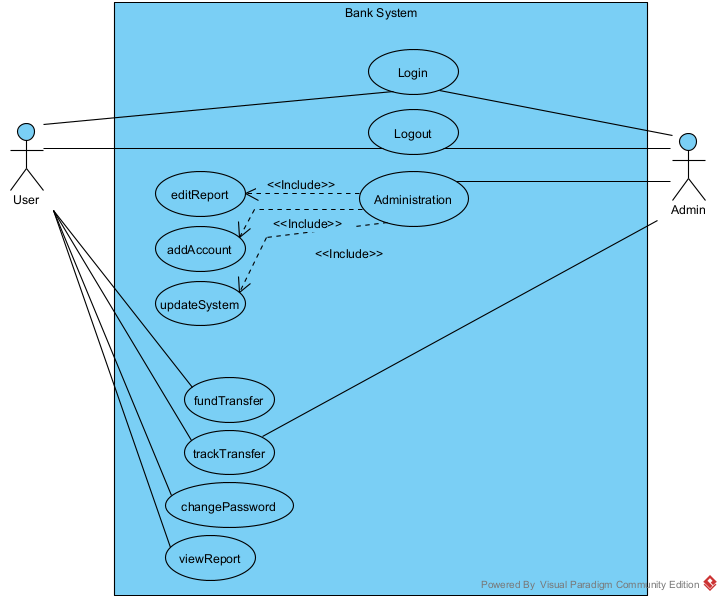
\includegraphics[width=\linewidth]{WeeklyReport/BankSysUseCase.png}
    \caption{Basic use case of banking system }
    \label{fig:usecase}
\end{figure}

As shown in Figure \ref{fig:usecase}, the banking system allows users and admins to log in and out, perform fund transfers, track transfers, change passwords, and view reports. Additionally, admins can perform administrative tasks such as editing reports, adding accounts, and updating system settings.

\newpage
\section{Class Diagram}

\begin{figure}[h]
    \centering
    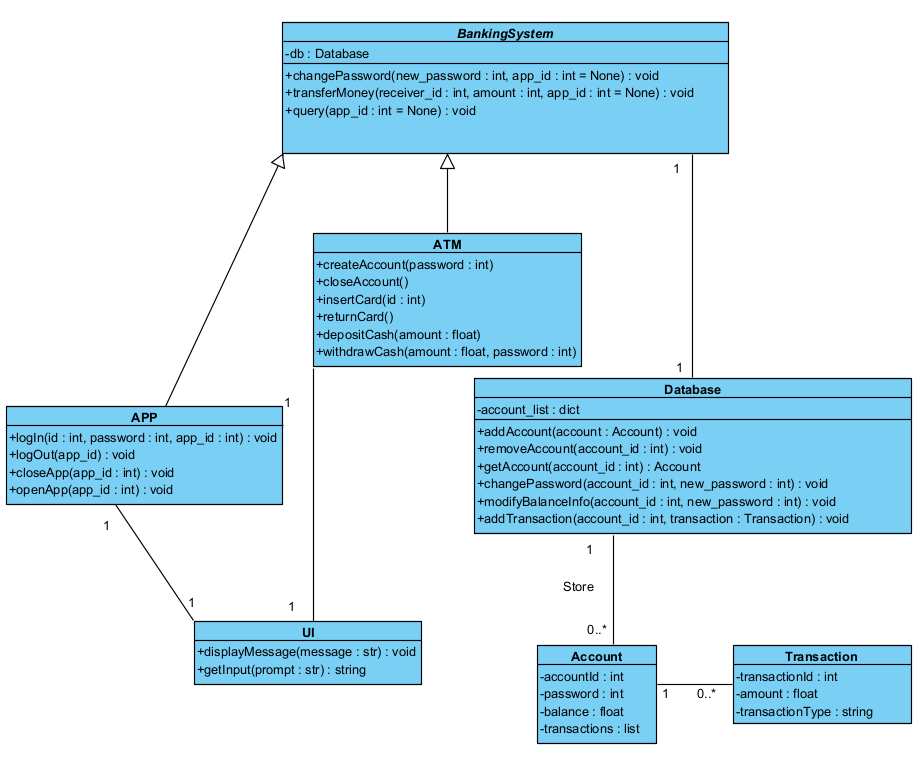
\includegraphics[width=\linewidth]{WeeklyReport/class_diagram.png}
    \caption{Basic class diagram of banking system }
    \label{fig:classdiagram}
\end{figure}

As shown in Figure \ref{fig:classdiagram}, the image is included and captioned correctly.
\end{document}